\documentclass[review]{article}

\usepackage{amsmath, amsfonts, amsthm} % Math packages

\usepackage{listings} % Code listings, with syntax highlighting

\usepackage[main = greek, english]{babel} % English language hyphenation

\usepackage{graphicx} % Required for inserting images
\graphicspath{{Figures/}{./}} % Specifies where to look for included images (trailing slash required)

\usepackage{booktabs} % Required for better horizontal rules in tables

\usepackage{dirtytalk} % Required for quoting.

\usepackage{float} % Added for hard placement of images.

\usepackage[dvipsnames]{xcolor} % Added for extra colors.

\usepackage{tikz} % For colored boxes and more.

\numberwithin{equation}{section} % Number equations within sections (i.e. 1.1, 1.2, 2.1, 2.2 instead of 1, 2, 3, 4)
\numberwithin{figure}{section} % Number figures within sections (i.e. 1.1, 1.2, 2.1, 2.2 instead of 1, 2, 3, 4)
\numberwithin{table}{section} % Number tables within sections (i.e. 1.1, 1.2, 2.1, 2.2 instead of 1, 2, 3, 4)

\usepackage[utf8]{inputenc} % Required for inputting international characters
\usepackage[T1]{fontenc} % Use 8-bit encoding

\usepackage{translator}

\newcommand{\en}[1]{\foreignlanguage{english}{#1}}
\newcommand{\src}[1]{{\texttt\en{#1}}}


% Extra Formatting

\setlength{\parindent}{0em}
\setlength{\parskip}{0em}


% Code Listing Style

\lstdefinestyle{code}{
  belowcaptionskip=1\baselineskip,
  breaklines=true,
  frame=LRTB,
  xleftmargin=\parindent,
  showstringspaces=false,
  basicstyle=\ttfamily,
  keywordstyle=\bfseries\color{green!40!black},
  commentstyle=\itshape\color{purple!40!black},
  identifierstyle=\color{black},
  stringstyle=\color{orange},
}


\newcommand{\lstcode}[3]
{
    \begin{otherlanguage}{english}
    \lstinputlisting[language=#2, frame=single, style=code, caption=#3]{#1}
    \end{otherlanguage}
}

\usepackage{lineno}
\usepackage{hyperref}
\modulolinenumbers[5]

\usetikzlibrary{positioning}

%% `Elsevier LaTeX' style
\bibliographystyle{unsrt}
%%%%%%%%%%%%%%%%%%%%%%%

\begin{document}

\begin{titlepage}

\title{Σχεδιασμός και υλοποίηση ψηφιακού ισοσταθμιστή ήχου.}
% \tnotetext[mytitlenote]{Fully documented templates are available in the elsarticle package on \href{http://www.ctan.org/tex-archive/macros/latex/contrib/elsarticle}{CTAN}.}

%% Group authors per affiliation:
\author{Ευάγγελος Λάμπρου}
\date{}

\maketitle

\begin{abstract}
    Στα πλαίσια αυτής της εργασίας γίνεται ο σχεδιασμός και υλοποίηση 
    ενός ισοσταθμιστή ήχου. 
\end{abstract}

% \begin{keyword}
%     \en{DSP}\sep \en{plguin}\sep ισοστάθμιση
% % \MSC[2010] 00-01\sep  99-00
% \end{keyword}

\end{titlepage}

\linenumbers

\section{Σχεδιασμός}

\begin{figure}[htpb]

    \begin{center}

        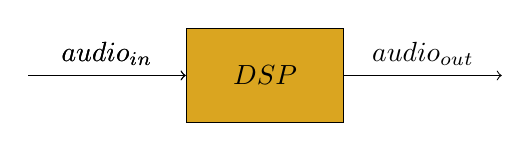
\begin{tikzpicture}

        % \node[draw,
        %     circle,
        %     minimum size=0.6cm,
        %     fill=Rhodamine!50
        %     ] (sum) at (0,0){};
        % \draw (sum.north east) -- (sum.south west)
        %     (sum.north west) -- (sum.south east);
        % \node[left=-1pt] at (sum.center){\tiny $+$};
        % \node[below] at (sum.center){\tiny $-$};

        % Controller

        \node [draw,
        fill=Goldenrod,
        minimum width=2cm,
        minimum height=1.2cm,
        right=1cm
            ] (dsp) {$DSP$};

        \draw[->] ++(-1,0) -- (dsp.west) 
            node[midway,above]{$audio_{in}$};

        \draw[->] ++(-1,0) -- (dsp.west) 
            node[midway,above]{$audio_{in}$};

        \draw[->] (dsp.east) --  ++(+2,0) 
            node[midway,above]{$audio_{out}$};
        \end{tikzpicture}
    \end{center}

    \caption{Βασική δομή του \en{plugin}.} 
\end{figure}

\begin{figure}[htpb]
    \centering
    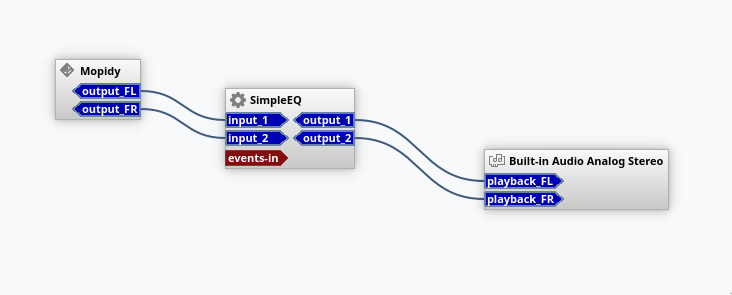
\includegraphics[width=0.8\textwidth]{./assets/Carla_Basic.png}
    \caption{Εφαρμογή του \src{SimpleEq plugin} στο περιβάλλον \en{Carla}.}
    \label{fig:carla_basic}
\end{figure}

\paragraph{Θεωρία \en{IIR} φίλτρων}
\paragraph{Φίλτρα \en{Butteworth}} 

\section{Υλοποίηση}

\paragraph{Γραφική Διεπαφή}
\paragraph{Χρήση}
\paragraph{Μετρήσεις}

\cite{Dirac1953888}

\bibliography{bibliography.bib}

\end{document}
